\chapter{Tehnologii folosite}

\section{Descrierea unei aplicații web}

O aplicație web poate fi manipulată direct online cu ajutorul unui browser web și nu trebuie instalată. Aceasta poate fi plasată și pe un server, iar accesul este simplu și se face prin intermediul unei rețele de calculatoare (internet, rețea locală etc.).\newline

O aplicație web dinamică constă într-un set de pagini statice și dinamice al căror conținut este parțial sau total determinat. Conținutul final al unei pagini este determinat numai atunci când utilizatorul solicită o pagină de la serverul web, iar aceasta variază de la o cerere la alta, în funcție de acțiunile utilizatorului.\newline

Spunem că o pagină web este statică dacă această pagină are un conținut fix și afișează acest conținut către toți utilizatorii.

În opozitie, o pagină web dinamică este mai complexă din punct de vedere tehnic, deoarece utilizează baze de date pentru a încărca informații, iar conținutul este actualizat de fiecare dată când utilizatorul se conectează la aplicație.\newline

Există multe limbaje de programare pentru dezvoltarea de aplicații web.
Asadar, pentru a programa această aplicație, am ales unul din cele mai populare framework-uri Java Enterprise Edition (Java EE), și anume, Spring, pe care îl voi prezenta ulterior.
\newline
\section{Generalități despre HTML}

HTML\footnote{Hyper Text Mark-up Language} este un limbaj de codare utilizat pentru a crea pagini pe care un browser web le poate afișa. Fișierele de tip HTML sunt alcătuite din elemente pereche, unul marcând deschiderea iar perechea sa, închiderea.\newline
Site-urile web sunt așadar compuse din diverse pagini HTML legate între ele, stocate undeva pe un server. De asemenea, acesta este motivul pentru care HTML este frecvent numit și "coloana vertebrală a internetului".\newline

Browser-ul folosit de către utilizatori este capabil, astfel, să interpreteze acest limbaj, fară să țină cont de majuscule sau minuscule, afișând rezultatul prin intermediul unei ferestre web.\newline\newline

\textbf{ Organizarea unui document HTML:}\newline
\lstset{frame=none}
\begin{itemize}
	\item
 \begin{lstlisting}[language=HTML]
  <html>  </html>
\end{lstlisting}
Acest tag reprezintă elementul de nivel superior sau rădăcina oricărui document HTML. Browser-ul înțelege prin intermediul acestui tag că este vorba de un fișier HTML pentru a-l putea afișa. De asemenea, toate celelalte tag-uri trebuie să fie descendente ale acestui tag.
	\item
\begin{lstlisting}[language=HTML]
  <head>  </head>
\end{lstlisting}
Între aceste tag-uri sunt conținute informații care pot fi citite automat (metadate) despre document precum titlul, script-urile, iar acestea vor fi prelucrate de browser.
	\item
\begin{lstlisting}[language=HTML]
  <title>  </title>
\end{lstlisting}
Aceste tag-uri sunt folosite pentru a da un titlu documentului. Astfel, acest text se va afișa în bara de titlu a browser-ului.
	\item
\begin{lstlisting}[language=HTML]
  <body>  </body>
\end{lstlisting}
Într-un document HTML, poate exista o singură astfel de pereche de tag-uri, ce reprezintă conținutul documentului care va fi afișat pe ecran.\newline
\end{itemize}
\section{HTML5}
A fost prezentat oficial publicului pe 22 ianuarie 2008, având următoarea actualizare majoră în octombrie 2014. Obiectivele acestui update au fost de a îmbunătăți limbajul cu suport pentru cele mai recente caracteristici multimedia și alte caracteristici noi, de a menține limbajul ușor de înteles atât de către oameni, cât și de către computere, fără rigiditatea XHTML-ului, dar și de a rămâne compatibil cu software-ul mai vechi.\newline

\textbf{ HTML4 vs HTML5 :}\newline

În comparație cu ediția anterioară de HTML, respectiv HTML4, au fost modificate în mod direct structura, echivalentă marcării, caracteristicile care permit redarea (culori, font etc.), echivalente cu directivele destinate stilului paginilor web și partea de conținut.\newline

HTML5 oferă totodată și o mai bună gestionare a erorilor și are o coerență ridicată în cazul documentelor malformate. De asemenea, versiunea nouă  oferă suport în ceea ce privește stocarea de cantități consistente, descărcate de pe web pe spațiul local de memorie, permițând astfel utilizarea offline unor aplicații web.
\newline

\section{Bootstrap}

Bootstrap este un framework de dezvoltare web gratuit și open-source, dezvoltat de Twitter în 2011 și lansat pe GitHub în același an, care reprezintă o colecție cu numeroase fragmente de cod reutilizabile și versatile scrise în CSS, HTML și JavaScript pentru a dezvolta rapid și ușor pagini web reactive.\newline
O pagină web reactivă este capabilă să se adapteze automat pentru a arăta mai bine în funcție de rezoluția sau dimensiunea ecranului ori aspectul de imagine.\newline

Așadar, folosind Bootstrap, se pot crea dropdown-uri, alerte, pop-up-uri, navigări etc.

\section{CSS}

CSS\footnote{Cascading Style Sheets} permite un control exact asupra aspectului elementelor HTML în browser, și astfel, se pot crea interfețe de utilizator reprezentative, fiecare pagină web putând avea un design unic. În CSS se poate defini dimensiunea, culoarea, poziția textului și a altor etichete HTML, în timp ce fișierele HTML definesc conținutul și organizarea acestuia.\newline

HTML poate defini atât structura, cât și prezentarea, dar WWW\footnote{World Wide Web} recomandă utilizarea CSS, pentru a separa structura unui document HTML de prezentarea sa, deoarece în loc să se definească stilul fiecărui bloc de text și al fiecărui tabel în HTML-ul unei pagini web, CSS sprijină dezvoltatorii front-end să creeze un aspect uniform ce se poate aplica pe mai multe pagini ale unui site web, definindu-le o singură dată într-un fișier/document CSS, având extensia specifică ".css".\newline

\section{Framework-uri în Java}
Obiectivul unui framework \cite{.javaframework} este, în general, de a simplifica munca dezvoltatorilor, oferindu-le o arhitectură "gata de utilizare" care să le permită să nu înceapă de la zero la fiecare nou proiect. Se prezintă într-o varietate de forme care pot include unele sau toate următoarele:

\begin{itemize}
	\item{Un set de clase grupate de obicei sub formă de biblioteci pentru a furniza servicii mai mult sau mai puțin sofisticate.}
	\item{Proiectare eficientă bazată pe modele de proiectare pentru a propune tot sau o parte din scheletul unei aplicații.}
	\item{Standarde de dezvoltare}
	\item{Diverse instrumente pentru a facilita dezvoltarea aplicației}
	\newline
\end{itemize}

Aplicația FitClub folosește 2 framework-uri Java pe partea de server, și anume Spring Boot și Hibernate.\newline


\subsection{Spring Boot}
Conceptul fundamental al Spring este injectarea dependențelor \cite{.javaspringbook}.
Acest framework a apărut ca răspuns la 3 factori de codare proastă, definiți în 1994 de Robert C. Martin, iar injectarea dependențelor este o soluție la această problemă:

\begin{itemize}
	\item{Rigiditate: este dificil să schimbi ceva, deoarece fiecare schimbare afectează prea mult funcționarea sistemului.}
	\item{Fragilitate: o modificare face ca funcționalitățile deja implementate care ar trebui să funcționeze corect să funcționeze defectuos.}
	\item{Imobilitate: este dificil de reutilizat codul într-o altă aplicație.}
	\newline
\end{itemize}

Spring Boot este, în principiu, o extensie a cadrului Spring, care elimină configurațiile de tip boilerplate necesare pentru configurarea unei aplicații Spring. Acesta adoptă o viziune avizată a platformei Spring, care deschide calea pentru un ecosistem de dezvoltare mai rapid și mai eficient.\newline

Așadar, pentru a crea o aplicație web folosind Spring Boot, avem nevoie de dependențe, unde folosim Maven pentru a le gestiona, aceasta fiind una dintre cele mai bine cunoscute caracteristici ale sale.\newline

Nu există mari dificultăți în gestionarea dependențelor pentru un singur proiect, dar atunci când avem de-a face cu proiecte cu mai multe module și aplicații formate din zeci sau sute de module, Maven poate ajuta la menținerea unui nivel ridicat de control și stabilitate.\newline

\subsection{Hibernate}

Datele sunt cel mai adesea stocate în baze de date relaționale, astfel încât se recomandă utilizarea unui framework de mapare Obiect/Relațional pentru a asigura viteza, scalabilitatea și mentenabilitatea dezvoltărilor. Hibernate\cite{.hibernate} răspunde acestei nevoi și are un mare succes de mulți ani. Acest succes poate fi explicat prin arhitectura sa, care este perfect adaptabilă la orice tip de dezvoltare și prin suportul pentru majoritatea bazelor de date.\newline

Hibernate este un framework de persistență utilizat pentru a gestiona persistența obiectelor Java într-o bază de date. Termenul de mapare\newline obiect/relațională (ORM) descrie tehnica de conectare a reprezentării obiectuale a datelor la reprezentarea relațională a acestora, pe baza unei scheme SQL.\newline

În termeni concreți, Hibernate permite ca un obiect definit în Java să fie legat/mapat la o tabelă dintr-o bază de date, prin intermediul unui fișier de corespondență declarativ. Sistemul se poate ocupa de crearea tabelelor în conformitate cu fișierele de configurare și, de asemenea, de actualizarea tabelelor, dacă este necesar, atunci când unul dintre fișierele de configurare se modifică.\newline

Hibernate are mai multe moduri de a efectua interogări. Este posibil să se exprime interogări în SQL sau în HQL\footnote{Hibernate Query Language: limbaj specific pentru limbajul propriu Hibernate}.\newline

\section{Funcționarea unei aplicații web}

Funcționarea unei aplicații web are la bază anumite mașini care comunică în rețea folosind un limbaj comun.
Dintre aceste mașini, se face o distincție între cele care oferă resurse, serverele, și cei care le folosesc, și anume utilizatorii finali sau clienții. Resursele pot fi, de exemplu, documente HyperText, imagini, fișiere XML sau chiar programe (PHP, Java) responsabile pentru generarea lor la cerere.\newline

Un server este un proces care execută o operație la cererea unui client și transmite răspunsul către client, care la rândul său este un procedeu care solicită executarea unei operații de la un web server process prin trimiterea unui mesaj care conține o descriere a operației care urmează să fie efectuată și așteaptă răspunsul la această operație printr-un mesaj de răspuns.
Atunci când un client accesează o resursă (consultarea unui document, modificarea datelor stocate pe server etc.), acesta trebuie să utilizeze protocolul de comunicare HTTP pentru a ajunge la aceasta: acesta definește o semantică foarte simplă (GET, POST și alte comenzi) care permite formularea de cereri care sunt interpretate pe server de un program specific, și anume, serverul web.\newline

Un server web este un simplu server de fișiere. Clienții i se adresează prin intermediul protocolului HTTP pentru a obține o resursă. Atunci când serverul web primește o astfel de cerere HTTP, acesta extrage pur și simplu numele resursei solicitate din cerere, apoi extrage resursa de pe disc și o împachetează într-un răspuns HTTP, pentru a o transmite clientului, fără a o prelucra înainte de a o transmite acestuia. Prin urmare, acesta poate transfera către un client o pagină HTML, o imagine, un sunet sau chiar un fișier executabil. Tipul de conținut al resursei solicitate este total irelevant pentru aceasta.
Atunci când un server web primește o cerere pentru o pagină web statică, acesta transmite această pagină direct către browserul care o solicită.\newline

Cu toate acestea, atunci când serverul web primește o cerere pentru o pagină web dinamică, reacționează diferit: transmite pagina către un software special care este responsabil pentru finalizarea paginii. Acest software special se numește server de aplicații.\newline

Un server de aplicații este radical diferit de serverul web, deoarece resursele care îi sunt oferite nu sunt doar fișiere statice, ci coduri pe care le va executa în numele clienților care le solicită. Atunci când un server de aplicații primește o cerere HTTP, acesta analizează și această cerere pentru a determina ce resursă este solicitată. De obicei, cererea este pentru un cod executabil găzduit de server. Spre deosebire de un server web aflat în aceeași situație, acesta nu transferă codul către client, ci îl execută, iar rezultatul acestui cod va fi returnat clientului.\newline

Server-ul de aplicații citește codul din pagină, completează pagina în conformitate cu instrucțiunile cuprinse în cod și ulterior, elimină codul. Server-ul de aplicații trimite înapoi la server-ul web rezultatul acestui proces care constă într-o pagină statică. La rândul său, trimite această pagină la browser-ul solicitant. Browser-ul primește, în consecință, doar cod HTML pur atunci când îi este trimisă pagina, pe care îl prelucrează corespunzător.\newline

Figura 2.1 prezintă o imagine de ansamblu a acestui proces:\newline

\begin{figure}[H]
	\begin{center}
		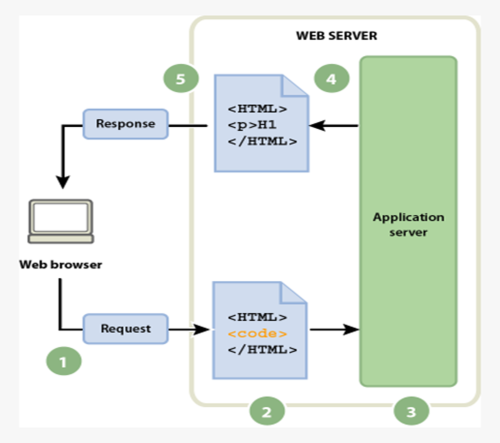
\includegraphics[width=9cm]{funct-app-web.png}
		\caption{Funcționarea unei aplicații web}
	\end{center}
\end{figure}

\textbf{Observație}: O resursă este identificată prin url (șir de caractere). Atunci când clientul dorește să ajungă la o resursă la distanță, acesta trimite o cerere HTTP în care menționează adresa URL a resursei.
\newline

\section{Arhitectura unei aplicații web}
\subsection{Arhitectura pe două niveluri (client/server)}
Arhitectura pe două niveluri numită și arhitectura "client-server" nu este deloc complicată. Pe de o parte se află clientul, iar pe de altă parte server-ul, așa cum este reprezentat și în Figura 2.2.\newline

Acest tip de arhitectură poate fi realizat pe orice tip de arhitectură hardware interconectată.

\begin{figure}[H]
	\begin{center}
		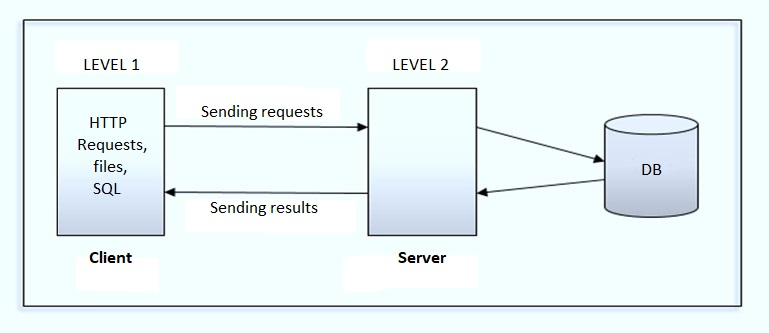
\includegraphics[width=13cm]{2level-arch.jpg}
		\caption{Arhitectura unei aplicații pe 2 niveluri}
	\end{center}
\end{figure}

Punctele importante ale unei aplicații pe două niveluri:

\begin{itemize}
	\addtolength{\itemindent}{1cm}
	\item[$-$]Clientul solicită un serviciu de la server, cum ar fi să i se afișeze o anumită pagină.
	\item[$-$]Server-ul primește această cerere HTTP, efectuează procesarea și returnează resursa solicitată de client.
	\item[$-$]Clientul primește resursa solicitată.
	\newline
\end{itemize}


\subsection{Arhitectura pe trei niveluri}
În arhitectura pe trei niveluri (Figura 2.3), apare un nou nivel. Într-adevăr, mai avem încă primul nivel, care este clientul, care este foarte ușor, deoarece nu are niciun rol de procesare, utilizează aplicația, dar are doar o mică parte a aplicației pe dispozitivul său de lucru.\newline

Toată procesarea se face apoi pe partea server-ului. La al doilea nivel se află server-ul de aplicații și, în sfârșit, la ultimul nivel, server-ul de baze de date, de unde se vor procesa anumite interogări SQL. Funcţia fundamentală a unui server de baze de date este reprezentată de: stocarea, regăsirea şi reactualizarea datelor. Pentru asigurarea acesteia, server-ul trebuie să ascundă față de utilizatorul care accesează site-ul, informațiile referitoare la implementarea fizică internă, cum ar fi detalii despre organizarea fișierelor, dar şi structurile de stocare.

\begin{figure}[H]
	\begin{center}
		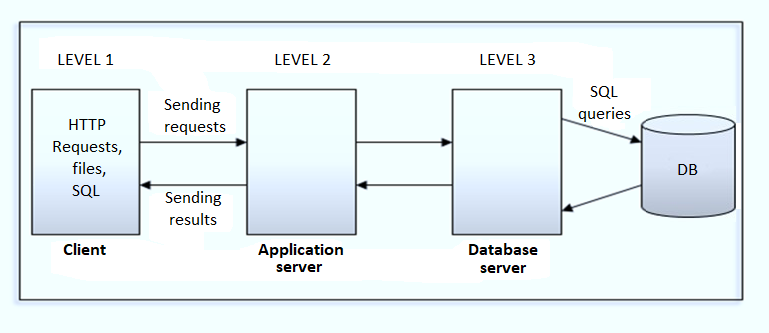
\includegraphics[width=13cm]{3level-arch.png}
		\caption{Arhitectura unei aplicații pe 3 niveluri}
	\end{center}
\end{figure}

Punctele importante ale unei aplicații pe trei niveluri:

\begin{itemize}
	\addtolength{\itemindent}{1cm}
	\item[$-$]Clientul este utilizat doar pentru a solicita și afișa răspunsurile serverului.
	\item[$-$]Server-ul de aplicații se ocupă de calcule și chiar solicită servere suplimentare.
	\item[$-$]Server-ul DB se ocupă de stocarea datelor.
	\newline
\end{itemize}

\section{Arhitectura Java EE}

Arhitectura Java EE se bazează pe o arhitectură stratificată, care se bazează pe o împărțire în straturi, astfel încât vorbim de aplicații pe mai multe niveluri. Astfel, sunt reprezentate trei straturi principale, în care sunt distribuite diferite componente pe care le vom vedea în restul acestui capitol.
Scopul acestei diviziuni este de a propune o mai bună distribuție a rolurilor (fiecare strat are un rol clar definit) și o mai bună mentenabilitate, având în vedere că fiecare strat este independent de celelalte.\newline
Are loc, așadar, următoarea împărțirea în straturi:

\begin{itemize}
	\item{Stratul destinat afișării paginilor web}
	\item{Stratul destinat gestionării logicii de afaceri}
	\item{Stratul destinat salvării informațiilor din baza de date}
	\newline
\end{itemize}

Stratul destinat afișării paginilor web gestionează afișarea datelor și interacțiunile aplicației cu utilizatorul. Separarea acestui strat face posibilă oferirea mai multor prezentări pentru aceeași aplicație: același strat de procesare poate fi utilizat pentru o aplicație grea și pentru o aplicație ușoară.\newline

Stratul destinat gestionării logicii de afaceri se referă atât la sarcinile care trebuie efectuate de aplicație asupra datelor, cât și la prelucrările necesare în urma unei acțiuni din partea utilizatorului: (verificarea stării utilizatorului: autentificat/neautentificat, diverse calcule etc.).\newline

Stratul destinat salvării informațiilor din baza de date (sistemul informatic al aplicației) grupează mecanismele de stocare și de acces la date, astfel încât acestea să poată fi utilizate de aplicație la nivelul de procesare.\newline


\section{Arhitectura MVC}
Majoritatea platformelor de dezvoltare a aplicațiilor web, inclusiv Java EE, nu impun o anumită ordine a codului, adică putem dezvolta în orice mod doriți. Problema este că, dacă dezvoltăm în orice mod, codul rezultat va fi nesatisfăcător din punct de vedere calitativ și va deveni dificil să găsim o bucată de cod sau o funcție pe care dorim să o modificăm.\newline
Pentru a evita această problemă, este recomandat sa utilizăm bune practici de dezvoltare numite Design Patterns. Un model de proiectare permite descrierea liniilor principale ale unei soluții.\newline

Modelul MVC descompune aplicația în straturi distincte și, prin urmare, are un impact puternic asupra organizării codului. MVC este acronimul de la Model - View - Controller. Practic, atunci când dezvoltăm o aplicație folosind arhitectura MVC, vom segmenta codul în trei părți sau straturi, fiecare strat având o funcție specifică.

\subsection{Stratul Model}
Aceasta este partea de cod care execută logica de afaceri a aplicației. Acest lucru înseamnă că este responsabil pentru recuperarea datelor, conversia lor în conformitate cu conceptele logicii aplicației, cum ar fi procesarea, validarea, asocierea și orice alte sarcini legate de manipularea datelor.\newline

Este, de asemenea, responsabil pentru interacțiunea cu baza de date, știe cum să se conecteze la o bază de date și să execute interogări, folosind cele patru operațiuni de bază ale stocării persistente (CREATE, READ, UPDATE, DELETE) pe o bază de date.

\subsection{Stratul View}
Aceasta este partea de cod care se va ocupa de prezentarea datelor către utilizator, care returnează o vizualizare a datelor din model, cu alte cuvinte, este responsabilă pentru producerea interfețelor de prezentare ale aplicației din informațiile pe care le deține (de exemplu, pagina HTML).\newline

Acest nivel nu se limitează însă doar la reprezentarea datelor în format HTML sau text, ci poate fi utilizat și pentru a oferi o mare varietate de formate, în funcție de ceea ce avem nevoie sa utilizăm pentru a implementa o anumită funcționalitate.

\subsection{Stratul Controller}
Acesta este stratul responsabil cu rutarea informațiilor, va decide cine va prelua informațiile și le va procesa. De asemenea, gestionează cererile utilizatorilor și returnează un răspuns cu ajutorul straturilor Model și View, descrise anterior.\newline

Figura 2.4 prezintă o imagine de ansamblu a arhitecturii MVC:\newline

\begin{figure}[H]
	\begin{center}
		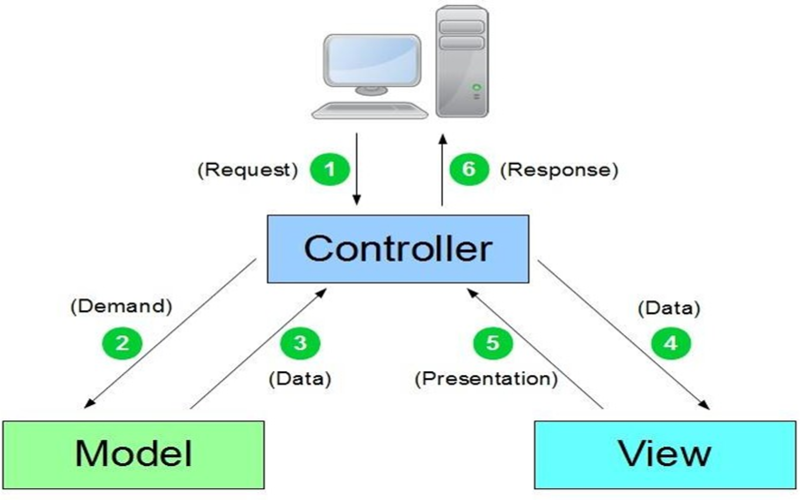
\includegraphics[width=9.5cm]{mvc-arch.png}
		\caption{Arhitectura Model - View - Controller}
	\end{center}
\end{figure}

Principiile arhitecturii MVC:

\begin{itemize}
	\addtolength{\itemindent}{1cm}
	\item[$-$]Utilizatorul trimite cererea HTTP, o transmite server-ului de aplicații care o transmite direct către partea de cod numită Controller.
	\item[$-$]Controller-ul se ocupă de direcționarea informațiilor, hotărând cine va prelua informațiile și apoi le va procesa, apelând, de fapt, modelul care conține informațiile structurate.
	\item[$-$]Modelul va efectua calcule sau prelucrări pe baza acestor informații și le va trimite înapoi la Controller.
	\item[$-$]Controller-ul va cere View-ului să genereze un View (pagină web).
	\item[$-$]View-ul generează o pagină web așa cum a fost solicitată de controller și o trimite către Controller.
	\item[$-$]Controller-ul primește pagina web pe care o va trimite utilizatorului, ca urmare a solicitării.
	\newline
\end{itemize}

\section{React}

React este o bibliotecă JavaScript open-source dezvoltată de Facebook începând din 2013, ce s-a axat pe crearea de interfețe pentru utilizator declarative folosind un concept bazat pe componente, în care fiecare componentă are propria stare.\newline
Dacă o componentă a paginii web tocmai a fost actualizată (de exemplu, dacă apăsăm pe un buton care declanșează apariția unui text pe pagină), acea parte este singura modificată de React fără a actualiza întreaga pagină. React utilizează "DOM virtual", care este o reprezentare a interfeței cu utilizatorul, stocată în memorie și sincronizată în mod constant cu "DOM-ul" real.\newline

Așadar, React nu este un framework, ci mai exact o bibliotecă, deoarece se ocupă doar de redarea interfețelor de utilizare și rezervă multe lucruri la discreția proiectelor individuale, putând fi considerată "View-ul" în modelul MVC. De asemenea, bibliotecile externe pot ajuta dezvoltatorul să utilizeze atât funcționalitățile HTML, cât și cele CSS și să le construiască în JSX.\newline

\textbf{Observație}: JSX este o sintaxă de extensie JavaScript utilizată în React cu scopul de a scrie cu ușurință HTML și JavaScript împreună.
\newline


Totuși, React are anumite limitări:

\begin{itemize}
	\item{Adesea, devine necesar ca anumite pachete să fie descărcate pe stația de lucru a dezvoltatorului pentru a putea accesa diverse funcționalități implementate deja în React}
	\item{Deși React suportă o mulțime de biblioteci externe, există foarte puține biblioteci native.}
	\item{Navigarea datelor în React este complicată și complexă, deoarece manipularea paralelă a datelor nu este suportată.}
	\newline
\end{itemize}

\section{JSON Web Token}
JWT\footnote{JSON Web Token}, este un mecanism utilizat pentru a partaja informații între două părți în siguranță - un client și un server. În cele mai multe cazuri, JWT este la bază un JSON codificat care conține un set de declarații și o semnătură. De obicei, este utilizat în contextul diverselor mecanisme de autentificare, pentru a partaja informații legate de utilizator. Este, de asemenea, o modalitate populară de autentificare/autorizare a utilizatorilor într-o arhitectură de microservicii.

Autentificarea JWT este un mecanism de autentificare fără stare, bazat pe token-uri, unde aceste token-uri, odată generate, nu mai pot fi modificate. Este utilizat în mod popular ca o sesiune fără stare bazată pe client, ceea ce înseamnă că serverul nu trebuie să se bazeze în totalitate pe un depozit de date sau pe o bază de date pentru a salva informațiile despre sesiune.\newline

JWT-urile pot fi criptate, dar de obicei sunt codificate și semnate. Scopul JWT-urilor semnate nu este de a ascunde datele, ci de a asigura autenticitatea acestora.\newline

Un JSON Web Token este împărțit în trei șiruri consecutive de caractere, separate print-un punct de suspensie:

\begin{itemize}
	\item{Primul șir reprezintă un Header, codificat în base64, în care se scrie tipul de token, algoritmul de semnătură utilizat etc.}
	\item{Al doilea șir de caractere va conține informațiile ce se doresc a fi reținute în componența token-ului pentru a fi utilizate ulterior, cum ar fi drepturile persoanei care deține acest token, etc. Aceste informații sunt structurate sub forma "subiect-informație": "informație-concretă". În acest context, apare noțiunea de "claims", ce reprezintă subiecte speciale care vor conține informații speciale, cum ar fi data de valabilitate a token-ului, numele serverului care a emis JWT-ul etc.}
	\item{Al treilea șir reprezintă semnătura. Scopul este de a concatena prima și a doua și apoi de a le hash-ui cu o cheie secretă. Astfel, este posibilă verificarea integrității token-ului, deoarece, dacă primul sau al doilea șir este modificat, al treilea șir nu va mai corespunde și se va ști că token-ul a fost modificat și, prin urmare, nu este valid.}
	\newline
\end{itemize}

Așadar, utilizarea unui astfel de mecanism de securitate devine relevantă în contextul protejării integrității informațiilor conținute în baza de date, deoarece fiecare utilizator primește un token unic în momentul autentificării pe site, ceea ce face ca utilizarea API-urilor disponibile de către orice altă sursă necunoscută să nu fie permisă.\newline

\section{MySQL}

MySQL este un sistem de gestionare a bazelor de date care permite stocarea datelor într-un mod structurat (bază de date, tabele, câmpuri, înregistrări etc.). Nucleul acestui sistem permite accesul la informațiile stocate prin intermediul unui limbaj specific numit SQL.\newline

Popularitatea MySQL este datorată, în special, de natura sa open-source, stabilitate, dar și de ușurința de utilizare și a performanței ridicate.\newline

\section{Git}

Git este un software descentralizat de control al versiunilor creat de Linus Torvalds, autorul nucleului Linux. Git poate fi descris ca un instrument de urmărire a conținutului utilizat în principal pentru a stoca cod datorită celorlalte caracteristici pe care le oferă. Acest cod stocat continuă să se schimbe pe măsură ce se adaugă funcționalități sau se modifică cele deja existente.\newline

Git are un depozit la distanță unde sunt stocate toate aceste informații și un depozit local care este stocat pe computer-ul fiecărui dezvoltator. Acest lucru înseamnă că varianta completă a codului unei aplicații nu există doar pe depozitul central, ci este prezentă pe toate computer-ele dezvoltatorilor care lucrează la aplicația respectivă.\newline

Așadar, un astfel de sistem de control al versiunilor ajută prin păstrarea unui istoric al modificărilor ce au avut loc de-a lungul dezvoltării aplicației.


\section{Editoare de cod sursă}
\subsection{Visual Studio Code}
În centrul său, Visual Studio Code oferă un editor de cod sursă foarte rapid, perfect pentru utilizarea zilnică. Cu suport pentru sute de limbaje, VS Code ajută prin caracteristicile sale, dar și prin mulțimea de extensii disponibile în Marketplace-ul integrat să menținem productivitatea la un nivel ridicat prin ilustrarea sintaxei, potrivirea corectă a parantezelor, indentare automată, selectarea fragmentelor de cod, a casetelor și multe altele. Scurtăturile de la tastatură sunt intuitive, datorită comunității numeroase de utilizatori care au contribuit cu astfel de sugestii, iar personalizarea ușoară a tuturor opțiunilor disponibile incluzând și schimbarea acestor scurtături de la tastatură, în funcție de propriile preferințe, permit navigarea extrem de ușoară și facilă prin codul aplicației.\newline

Menționăm câteva dintre caracteristicile unice ale Visual Studio Code:
\begin{itemize}
	\addtolength{\itemindent}{1cm}
	\item[$-$]Include un suport încorporat îmbogățit pentru dezvoltarea Node.js cu JavaScript, având instrumente excelente pentru tehnologii web, cum ar fi JSX/React, HTML, CSS, Bootstrap.
	\item[$-$]Include suport încorporat pentru finalizarea codului, numit IntelliSense, folosit așadar pentru înțelegere și navigare semantică bogată a codului și refactorizare a codului.
	\item[$-$]De obicei, suportă toate limbajele de programare, dar, dacă se dorește utilizarea unui limbaj de programare care nu este acceptat, atunci se poate descărca și utiliza o extensie.
	\item[$-$]Include suport pentru Git, astfel încât se poate sincroniza în timp real cu sistemul de control al versiunilor fără a părăsi editorul, inclusiv vizualizarea modificărilor în așteptare.
	\newline
\end{itemize}



\subsection{IntelliJ IDEA}
IntelliJ este unul dintre cele mai puternice și populare medii de dezvoltare integrată (IDE) pentru Java. Este dezvoltat și întreținut de JetBrains și este disponibil în edițiile Community și Ultimate. Acest IDE bogat în funcții permite dezvoltarea rapidă și ajută la îmbunătățirea calității codului. Algoritmul său predictiv poate presupune cu exactitate ceea ce un dezvoltator încearcă să tasteze și astfel, devine reprezentativă utilitatea acestei funcționalități prin diversele sugestii ce sunt afișate, chiar dacă nu cunoaște numele exact al unei anumite clase, membru sau orice altă resursă.\newline

Menționăm, așadar, câteva dintre caracteristicile productive de top ale IntelliJ IDEA:
\begin{itemize}
	\addtolength{\itemindent}{1cm}
	\item[$-$]Suportă completarea inteligentă a codului bazată pe context. Oferă o listă cu cele mai relevante simboluri aplicabile în contextul curent.
	\item[$-$]Suportă completarea codului în lanț care este o funcție avansată ce listează simbolurile aplicabile accesibile prin metode în contextul curent.
	\item[$-$]Permite utilizarea de metode sau constante statice, și adaugă automat declarațiile de import necesare pentru a evita erorile de compilare.
	\item[$-$]Găsește din mers fragmentele de cod duplicat și oferă utilizatorului o notificare/sugestie în acest sens.
	\item[$-$]Capabil să detecteze în timp real o posibilă greșeală, fie că vorbim despre o greșeală de scriere, sau accesarea unei variable/metode inexistente sau orice altă situație ce poate genera eroare de compilare, caz în care o mică notificare cu beculeț apare pe aceeași linie.\newline Inspectând această notificare, se afișează o listă de sugestii prin care dezvoltatorul poate remedia rapid greșeala.
	\newline
\end{itemize}

\section{Găzduirea aplicației pe Microsoft Azure}

Microsoft Azure pune la dispoziție un abonament destinat studenților care oferă 100 de dolari în credite Azure ce pot fi folosite pentru a accesa diverse servicii\footnote{Azure App Services} Azure, fără a fi nevoie de un card de credit la înscriere. Printre aceste servicii, se numără și posibilitatea de a găzdui o aplicație web.\newline

Ca resurse principale, Microsoft Azure se bazează pe serviciile descrise anterior, în scopul găzduirii aplicațiilor web și a API-urilor web pentru orice platformă sau dispozitiv, și nu numai\cite{.azure}.\newline

Pentru găzduirea platformei FitClub au fost necesare doua astfel de servicii Azure: unul pentru API-urile web, și unul pentru aplicația client-side. De asemenea, persistența datelor este asigurată și în acest caz, prin folosirea unui serviciu Azure care permite rularea unei instanțe de baze de date relaționale, numit Azure Database for MySQL: Single Server. Toate aceste servicii sunt definite în cadrul unui grup de resurse.\newline

Aplicațiile sunt găzduite în planurile App Service, care sunt create într-un App Service Environment. Un App Service Plan este, în esență, un profil de planificare și configurare pentru găzduirea unei aplicații.\newline

Fiecare aplicație, fie că este o aplicație web sau o aplicație ce implementează API-uri web, funcționează pe baza unui App Service Plan, fiind, de asemenea, limitată la puterea de calcul a acelui hardware dedicat, numit gazdă, care diferă în funcție de abonamentul și configurările specifice fiecărui utilizator\cite{.azurebook}.\newline

\textbf{Observație}: Serviciul Azure responsabil pentru rularea unei instanțe de baze de date relaționale ce a fost descris anterior, nu are nevoie să opereze în cadrul unui App Service Plan.\newline\newline

Pentru găzduirea aplicației ce implementează API-urile web, este necesară generarea unor artefacte, folosind în terminal comanda \code{mvn clean install}. Concret, se generează un fișier cu extensia .jar, după rularea cu succes a tuturor testelor și curățarea tuturor rezultatelor compilărilor anterioare. După aceea, sunt necesare câteva configurări adiționale în cadrul proiectului care vor fi folosite pentru a încărca aplicația cu succes pe Microsoft Azure.\newline

Pentru găzduirea aplicației client-side, este necesară crearea unui director ce conține versiunea de producție a aplicației, prin rularea în terminal a comenzii \code{npm run build}. Acest director va conține un set minimal de fișiere ce vor putea fi copiate în cadrul oricărui server web și care vor acționa ca aplicația client-side propriu-zisă.\newline

De asemenea, sunt necesare configurări adiționale în cadrul aplicației client-side pentru a putea accesa endpoint-urile corespunzătoare aplicației ce implementează API-urile web.

\label{chap:02}